\documentclass[a4paper]{article}
\usepackage[no-math]{fontspec}
\usepackage{amsmath}		% /nonumber
\usepackage{xeCJK}
% \setCJKmainfont[BoldFont=SimHei,ItalicFont=TW-Kai]{SimHei}
\setCJKmainfont[Script=CJK]{SimHei}
% \setCJKfamilyfont{SimSun}
% {AR PL KaitiM GB}
% \setCJKfamilyfont{songvert}[Script=CJK,Vertical=RotatedGlyphs]{SimSun}
\xeCJKsetup{CJKecglue = {\hskip 0.2em plus 0.02em minus 0.01em},
	xCJKecglue = {\hskip 0.2em plus 0.02em minus 0.01em}}

\usepackage[a4paper,margin=0.5in,footskip=0.2in]{geometry}

%\usepackage{zxjatype}
%\usepackage{flowfram}
%\newflowframe{\textheight}{\textwidth+2em}{0pt}{\textheight}[mainframe] 
%\setflowframe{1}{angle=-90} 

\usepackage{parskip}
\setlength{\parskip}{1em} % 1ex plus 0.5ex minus 0.2ex}
\lineskip=0.5em

\title{威尔基$\cdot$柯林斯和他的《白衣女人》}
\author{朱虹, 2015}
\date{}

\begin{document}
\maketitle

\begin{equation}
\nonumber
\vcenter{\hbox{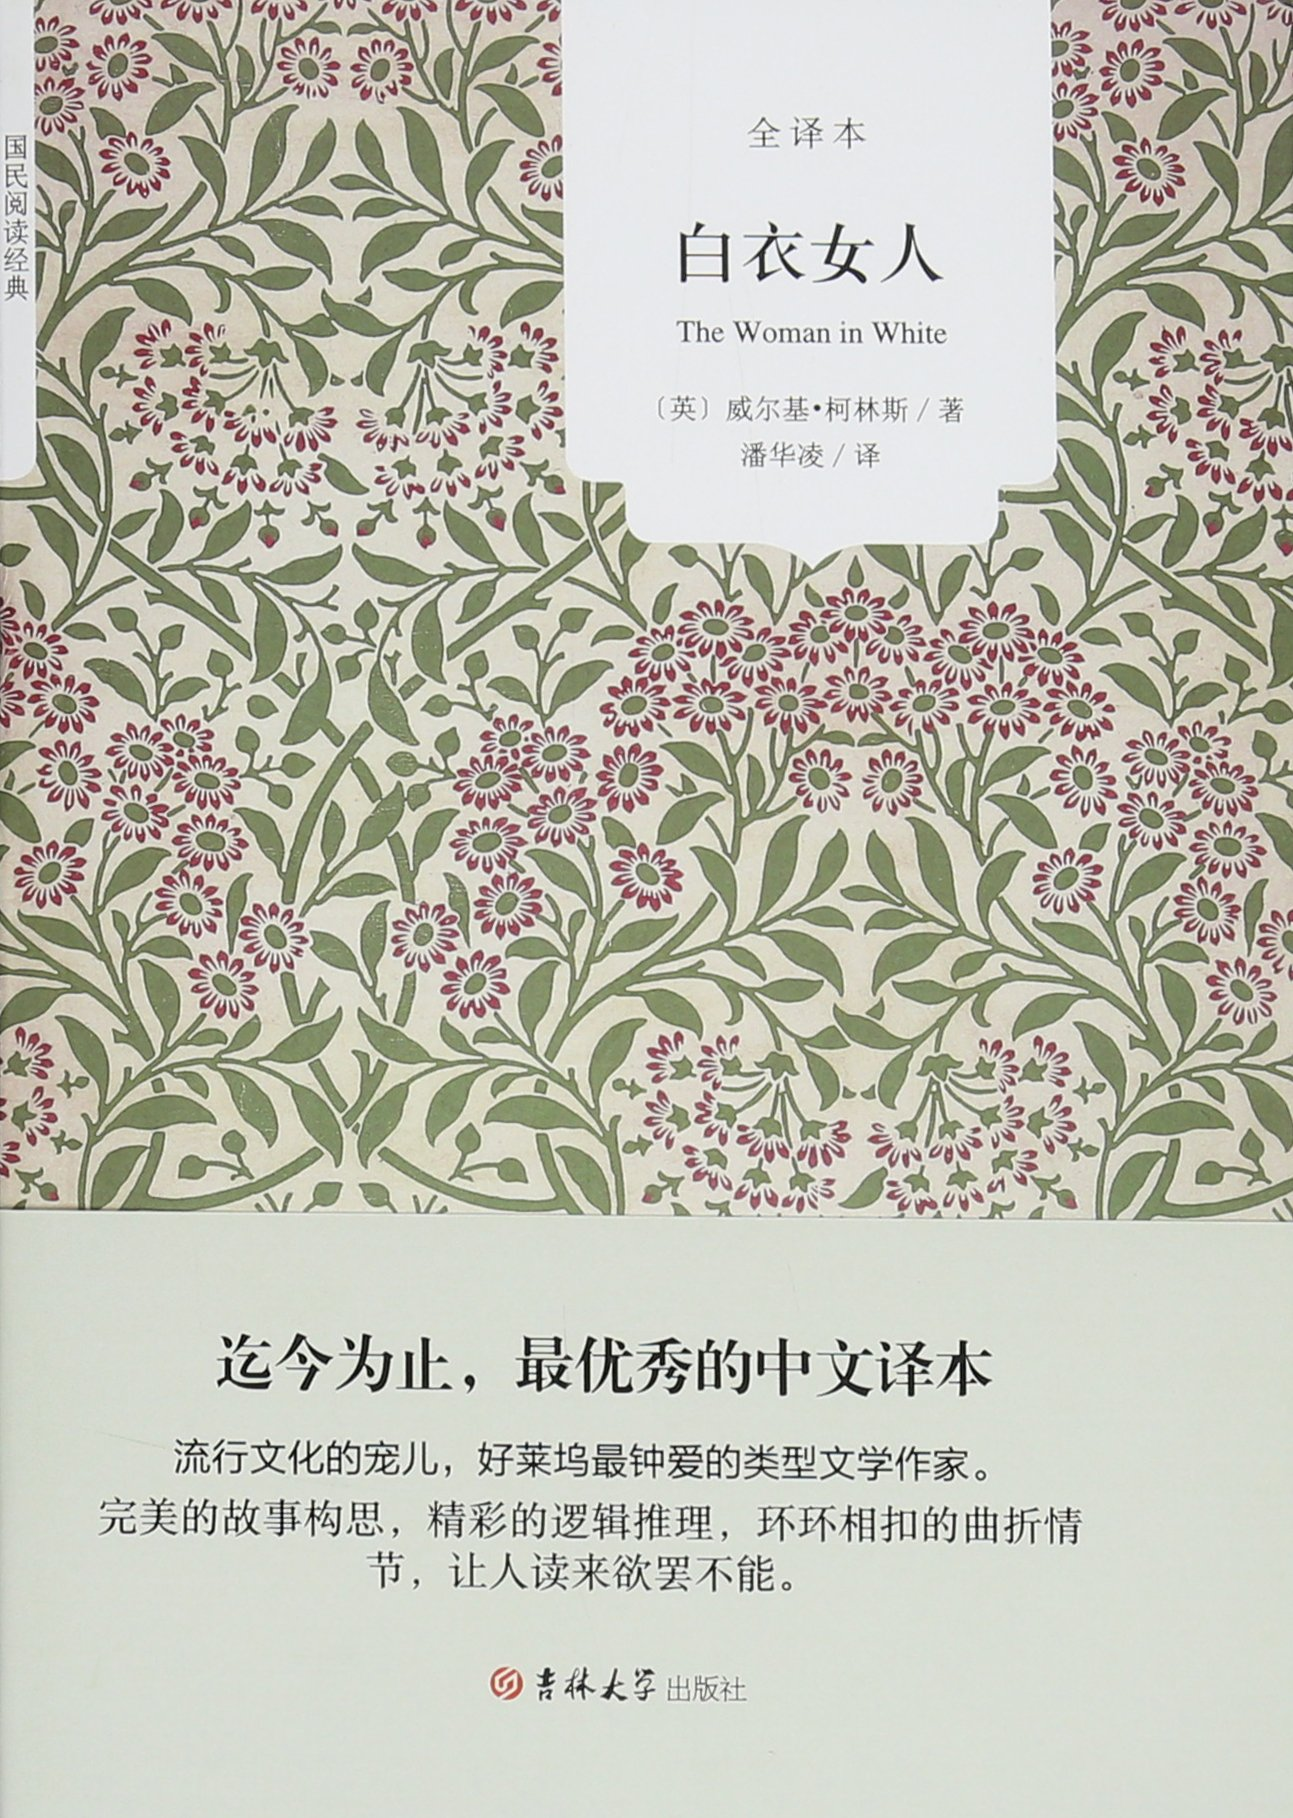
\includegraphics[scale=0.25]{woman-in-white-cover1.jpg}}}
\end{equation}

\section{柯林斯其人}

凡提起 19 世纪英国小说高峰,人们一般总是想起狄吏斯、萨克雷、勃
朗特等作家。 实际上,还有一个威尔基 $\cdot$ 柯林斯 (Wilkie Collins,1824-
1889) 不可忽视。 柯林斯生前在大众读者中间享有盛名,某些作品的销路
甚至超过狄吏斯。 他去世后被评论界贬为通俗写作家,但近年来又被重
新发现。 柯林斯最新传记的作者描述了这个转变过程。 她说: 他当年的
朋友会惊讶地发现,他的作品再一次被严肃认真地对待。 他去世以后,他
的作品虽然保持稳定的销路。 《白衣女人》的第六版据称卖了 30 万册,
但是他的大部分作品显得过时了,无足轻重。 在很长的一段时间里,人们
只知道他是《月亮宝石》和《白衣女人》的作者、一位卓越编造故事情节的
巨匠、侦探小说之父。 可是一百年后的今天,他的作品身价百倍。 它们使
我们窥见维多利亚时代生活表层底下的怪异和激情。

``柯林斯本人曾公开冒犯当时的伦理规范而不以为耻。 因此,他所
揭示出的自己时代的阴暗面,既离奇又令人着迷,在当时的小说林里是
无与伦比的。 维多利亚时代当然产生过更伟大的作家,但是威尔基 $\cdot$
柯林斯是独一无二的。" \footnote{D 加瑟琳 $\cdot$ 彼特斯: (故事大王 --- 威尔基 .柯林斯传), 塞克与沃伯格,伦敦 1991 年版. 第 434 页。 --- 译者注}

当前,柯林斯的研究十分兴旺发达。 自从 20 世纪 50 年代出版了几
部传记以来,英国和美国都陆陆续续有新传出版。 特别是随着现代心
理学理论和女权主义在文艺批评巾的影晌,随着通俗文艺研究作
为一个学科的建立,柯林斯的创作吸引着越来越多的学者开辟新的研
究领域.使柯林斯成为当前英国19世纪小说研究中的一个热点。

威尔基 $\cdot$ 柯林斯的一生就像个故韦。 柯林斯家族似乎有艺术基
闪,儡也的祖父是爱尔竺后裔,以经菅艺术品为生。 威尔基 ' 柯林斯的父
亲咸廉一柯林斯是位…玩家,在当时小有名气。 柯林斯的弟弟查尔斯继
承父业,只不过才艺不高,除了他给哥哥做的画像流传下来,他没有留
卜ˉ儡卜么儡乍品。 唯有长子威尔基.柯林斯不让父母省心。 十七岁时,威
尔基的父亲把他送到一家茶叶迸口商的办公室学生意。 学生意不成,
五年以后臧尔基又去学法律。 实际上他是在秘密地从事创作。 老柯
林斯去世后臧尔基放下「丨己的创作,写了一部关于父亲的《回忆录》。
《间忆录》出版后获得好评,威尔基 一 柯林斯意想不到地成为作家了。
他被伦敦的文艺圈子接纳为知己戒为狄更斯的密友,并逐渐进入自己
创作的黄金时代浔出了他的几部代表性作品,主要是长篇小说《巴西
尔,当代生活故事》(邝SZ)、《捉迷藏》(1854)、《绝密》(1857)、《白衣女
人》(丨860)、《无名无姓》(1862)、《阿玛戴尔》‖866)、《月亮宝石》
(1868)等等。 他共写出30余部长篇小说,此外还有许多短篇小说和戏
剧作品,其中有一部分是与狄吏斯合作的。

威尔基-柯林斯从青年时期便是反叛者。 他在自己的那些情节曲
折、扣人心弦的故事里抨击社会不平;他利用自己的法律知识,揭露当
时许多法律条文的不合理,特别是那些涉及妇女、非婚生子女或弱智人
权益方面的法律。 对妇女地位和权利的关心贯穿他的全部著作。 柯林
斯笔下的妇女形象,无论是受迫害的“白衣女人”,还是“无名无姓”的
复仇女神麦达琳,都从正面或反面强烈地提出了女性的地位和权利问
题。 柯林斯也最早揭开家庭内幕,让其中的性暴力和种种罪恶与丑闻
赚光。 这还联系到柯林斯作品中的另一个重要特点,即他对一切隐蔽
的神秘的东西和反常、病态心理的特殊兴趣。 他的许多作品中都有一
个白我确认的问题一一“我是谁?”也就是说,他的那些跌宕情节的背后
是人心的秘密和人的复杂性。 总之,柯林斯在 l9 世纪的小说家中,可
以说是位超前的人物。

威尔基 ' 柯林斯自己的生活也不无神秘色彩。 他生活中最有名的一
段掏…足携名则家约翰 ˉ 米莱的儿扦「1899年的《测忆求》巾第一一-次披
露的u 作拧称这足他父亲肥州看诉他的: 有铡天晚.. 柯林斯兄弟二人和
米莱 起I‖过晚餐后陪神米莱步行回家。 将他订潞过一座花园住宅的满
墙时,突然听到电而传出一声尖叫,接若一个身若门衣的年轻女人破门血
…,她在宅位男七而前停住,瞬间又迅速顺裨犬路跑远,白衣在月光下一
闪一闪的。 “多么美的女人哪!”米莱叫道。 “我得去看个究竟!"柯林斯
说若就追 去,也消失在月夜里。 根据《回忆录》和柯林斯的弟弟查尔斯
的妻子(狄更斯的女儿)的记载,这个神秘的口衣女人是加罗琳-格雷夫
斯,日那次传奇般的相遇后便成为柯林斯的终身伴侣。 更奇特的是,柯林
斯在惰加罗琳同居期佩丨司时还另有一个非正式家庭。 玛莎 '路德与柯
林斯同居多年,并为他生了三个孩子。 在当时的维多利亚社会,这种关系
不为社会所容,因此柯林斯自己实际上过着三重生活。 一方面他是著名
作家,与社会名流来往频繁.这是他的公开身份;另一方面他同时又分别
跟两个情妇过着一种秘密生活。 因此,“我是谁”的自我确认间题始终伴
随着柯林斯,并对他的创作中产生了深深的影响。
《白衣女人》的另一个来源是法国一桩掠夺财产公案的记载。 早在
1939 年克莱德 - K - 海德在他的〈威尔基 ' 柯林斯和〈白衣女人〉》一书
中就已披露了有关材料。 1856 年柯林斯与狄更斯同游巴黎时在一个书
摊上买了一本梅冉著的《著名案例纪实》,其中杜欧夫人的冤案,在每个
关键地方都与“白衣女人"的故事吻合:一个穿着白衣的女人被麻醉,关
进疯人院,被冠以别人的名字与身份,后来被宣布死亡以便她的财产可
以被吞食 ------ 柯林斯自己从不讳言他从梅冉记录的案件中得到启发。
总之,“白衣女人”在月夜里的闪现,改变了柯林斯的一生,并启发
他写出他的第一部传世之作。 柯林斯死后,根据他自己的遗嘱,他的碑
上只刻下“威尔基 '柯林斯,《白衣女人》的作者”几个字,别无其他,足
见《白衣女人》和“白衣女人”在柯林斯向己生活和创作申的地位。

\section{独一无二的故事大王}

《白衣女人》首先在狄更斯的刊物《一年四季》上分期连载。 每逄
新的一期要出版,读者都蜂拥而至,抢购一空。 成书后,《白衣女人》仍
然是畅销书、社交场合的热门话题。 商人用“白衣女人"做招牌,一时

问,“门衣女人”香水、“白衣女人”披肩、“白衣女人”华尔兹乐曲等充斥
巾场,形成一股白热化的“口衣女人”热。

《白衣女人》的出版之所以如此轰动,首先还是因为它的情节引人
入胜。 以身着白衣的女人在月光下闪现开始,《白衣女人》被誉为整个
英闰小说文学中最别出心裁、最组织严密、最夭衣无缝的布局。 正面女
主入公劳拉一费尔利美丽、善良而富有,是个标准的女主人公。 劳拉婚
姻不幸,她的丈夫珀西瓦尔 一 格莱德爵士冷酷而野蛮,一心想要夺取她
的财产。 伙同珀西瓦尔作恶迫害劳拉的是有意大利血统的福斯科伯爵
夫妇。 另一方面,标准的男主人公,具有骑士风度的沃尔特 一 哈特莱特
默默地爱着劳拉她与劳拉同母异父的姐姐玛丽安 一 哈尔寇姆齐心协
力为保护劳拉而与两个坏蛋展开了善与恶的大搏斗。 这场斗争牵涉到
当时的政治、法律、继承权及社会习俗的许多方面,紧张而曲折。 “白衣
女人”穿梭于故事中,增加了神秘色彩。 这个“白衣女人”到底是谁? 珀
西瓦尔爵土为什么要跟踪迫害她? 这个“白衣女人”与女主人公劳拉是
什么关系一两个人相貌酷似,而且都只穿白色的衣服? 从这个意义
上说,这部小说简直应该叫作《白衣女人们》。

《白衣女人》不是一个疑案,而是层出不穷的疑案。 它令人着迷不
仅在于破案过程的悬念与刺激,更在于阴谋的策划和阴谋的挫败像一
幕一幕的戏在读者眼前展开,其中许多场面令人难忘。 臼衣女人在洒
满月光的大路上出现是英国小说中一个著名的开场。 狄更斯认为它是
文学史上最具有戏剧性的两个场面之一,另一个是卡莱尔《法国大革
命》一书中关于妇女队伍进军凡尔赛的描写。 此外,劳拉在自己墓碑后
面像个幽灵似的出现,两个死敌沃尔特和珀西瓦尔爵士在偏僻乡村古
教堂里做殊死的较址以及后者葬身火海等都是《白衣女人》中描写得
惊心动魄的场而。

在形式上,《白衣女人》也不同于一股。 柯林斯采取让众多人物分
头提供“证词”的叙述方法是有他的用意的。 有一次他在法庭旁听,看
到证人一个个出庭做证,得到启发,便决定把自己隐匿起来,让故事中
的人物分头用自己的语言叙述所闻所见〇。 他在《白衣女人》前言中说

(D N. P. 戴维斯:(威尔基 一 柯林斯),第z‖ 页。 一译者注

帅],“门衣女人”香水、“门衣女人”披肩、“口衣女人”华尔兹乐曲等充斥
巾场 , 形成一股 白 热化的 “ 口 衣女人” 热。

《门衣女人》的出版之所以如此轰动,首先还是因为它的情节引人
入胜。 以身着白衣的女人在月光下闪现开始,《臼衣女人》被誉为整个
英闰小说文学申最别出心裁、最组织严密、最天衣无缝的布局。 正面女
主人公劳拉 . 拙尔利美丽、善良而富有,是个标准的女主人公。 劳拉婚
姻不幸,她邮J丈夫王白西瓦尔 '格莱德爵士冷酷而野蛮,一心想要夺取她
的财产。 伙同珀西瓦尔作恶迫害劳拉的是有意太利血统的福斯科伯爵
夫妇。 另一方面,标准的男主人公,具有骑士风度的沃尔特 一 哈特莱特
默默地爱着劳拉,他与劳拉同母异父的姐姐玛丽安 - 哈尔寇姆齐心协
力为保护劳拉而与两个坏蛋展开了善与恶的大搏斗。 这场斗争牵涉到
当时的政治法行只继承权及社会习俗的许多方面,紧张而曲折。 “白衣
女人”穿梭于故事中,增加了神秘色彩。 这个“白衣女人”到底是谁? 珀
西瓦尔爵士为什么要跟踪迫害她? 这个“白衣女人”与女主人公劳拉是
什么关系一两个人相貌酷似,而且都只穿白色的衣服? 从这个意义
上说,这部小说简直应该叫作《白衣女人们》。

《白衣女人》不是一个疑案,而是层出不穷的疑案。 它令人着迷不
仅在于破案过程的悬念与刺激,更在于阴谋的策划和阴谋的挫败像一
幕一幕的戏在读者眼前展开,其中许多场面令人难忘。 白衣女人在洒
满月光的犬路上出现是英国小说中一个著名的开场。 狄更斯认为它是
文学史上最具有戏剧性的两个场面之一,另一个是卡莱尔《法国大革
命》一书中关于妇女队伍进军凡尔赛的描写。 此外.劳拉在自己墓碑后
面像个幽灵似的出现,两个死敌沃尔特和珀西瓦尔爵士在偏僻乡村古
教堂里做殊死的较址.以及后者葬身火海等都是《白衣女人》中描写得
惊心动魄的场面。

在形式上,《白衣女人》也不同于一般。 柯林斯采取让众多人物分
头提供“证涮”的叙述方法是有他的用意的。 有一一次他在法庭旁口斤.看
到证人一个个出庭做证,得到启发,儡更决定把日己隐匿起来,让故事中
的人物分头用自己的语言叙述所闻所见@。 他在《口衣女人》前盲中说

〇 N~ P. 戴维斯:(威尔基 一 柯林斯),第2‖ 页。 一译者注

道:“‖言如法官升堂听「二丨供,现在读者也来坐堂了。”在《白衣女人)中.
各个人物从不同角度对问一个事件提供完全不同的“证词”,这就为塑
造性格而开辟了艺术空间。 不仅如此,上升到理论上去看,这种叙述方
法还暗示了真理的相对性和“知识”的不可靠性。
特别需要指出的是“知识”、信息,在《白衣女人》故事发展中的关
键作用:珀西瓦尔爵士无情地迫害“口衣女人”,是误以为她手中掌握
“知识” 一他的不可告人的秘密。 福斯科伯爵不遗余力地迫害劳拉,
欲置其于死地,不仅仅是指望从她丈夫手里分得钱财,他主要是怕劳拉
知道他的真正身份。 如此蔓延开去,又派生出 r新的间题.即女人掌握
“知识”就构成了对男人的威胁 ------
在《白衣女人》巾,挫败坏人的阴谋也是一个积累“知识”的过程:
日记、信件、回忆等都提供了导向破案的信息。 在这个间题上,双方有
几个回合。 玛丽安偷听了珀西瓦尔爵士和福斯科的阴谋,在这场较量
中,暂时占了上风。 但福斯科乘玛丽安病重神志不清的当JL儡俞看了她
的日记,得到了新的信息,结果又赢回了主动权。 在制造阴谋和挫败阴
谋的较量中,“知识”是争夺的对象,在斗争双方之间来回换手。 最后,
男主人公沃尔特掌握了全部“知识”、全部信息,因此能做到拯救劳拉、
澄清“白衣女人”的疑案并获得最后胜利。 沃尔特的胜利不在于他的道
德优势,而是决定于他掌握的“知识”所负载的隐秘信息,持别是决定于
他运用“知识"的技巧和能力。 如前所述,(白衣女人)中特殊的叙述方
式意味着真理的相对性。 可是另一方面.我们也看到,(白衣女人)特殊
的破案方式又指向另一个真理,即“知识就是力蹴”。 在这里,技巧、形
式、性格描写与哲理性都融为一体了。
总之,柯林斯是编造惰节、摆开场面、制造气氛、控制读者和寓哲理于
情节中的高手。 他被同代人誉为“故事大干”,并不包含任何贬意因为一
个能抓住读者的好故事是评价小说成败的重要标准,起码在当时是如此。
威尔基 -柯林斯最憧得掌拥读者心理.帷得图书市场的微妙层次。
掘传,“让他们哭! 让他们笑! 让他们等广的名言使是柯林斯对狄更斯的
“献策”。 柯林斯有一篇文章(论无名的大众),对通俗作家与大众读者的
互相关系有精辟的分析:“一个巨大的读者群被发现了。 下一一一步是 ------ 教
给这个读者群如何读书 ------ 要说英国小说的未来取决于这个无名的读霜ˉ

群并不过分 ------ 一个伟大耐空前的前景等待着下一代英国小说家。 发现
这…读者群的功劳要归于廉价的通俗读物,一旦这个读者群自己发现他
们黯要一个伟大的作家,那位作家会应运ˉ丨flˉ]ˉ生并获得空前的读者。”
(丨858)共实没有等到下一代,柯林斯自己的《白衣女人》就获得巨太的成
功赢得了这个无名的读者群。 在《白衣女人》出版的l9 世乡己60年代,图
书巾ˉ场正在形成,成百成千的小说畅销一时便销声匿迹。 《白衣女人)却
流传下来,一代一代的读者从中发现新的乐趣和新的意义。
三 “自家门口"的黑暗与恐怖

从故串的结尾看《白衣女人》,其总的倾向是保守的。 珀西瓦尔爵
士非法占有的黑水庄园回到了合法继承人的手里,而劳拉的小儿子被
确立为利默里奇庄园的继承人。 也就是说,全书以确立正统道德与合
法财产继承杈而达到完满的终点,呈现出一个善恶分明的光明世界。

然而这光明只是表面,下面隐藏着一个是非颠倒、道德沦丧的“反
世界”。 《白衣女人》的故事主要发生在两处庄园。 在英国的小说传统
中,庄园向来被视为历史、文化、传统的象征,如《傲慢与偏见〉中的彭伯
利庄园傲然立于祖传的土地上,不仅掌握地方上的政治经济命脉,而且
有丰富的藏书与绘画,是远近知名的文化中心。 19 世纪40年代,勃朗
特以《简 - 爱》推翻了庄园的神圣性,掀开了其屋顶,提出一个阁楼里的
疯女人及世家望族的丑闻。 《白衣女人》的故事也以庄园为主要背景:
劳拉娘家的利默里奇庄园和夫家的黑水庄园。 第一眼看上去,这两个
处所都是古老的宅邸,依山傍水,i丕有大片的树林和恬静的庭院。 可是
其巾潜藏的威胁很快便暴露出来。 玛丽安第一次脚踏黑水庄园时就碰
到许多不祥的预兆:湖边的蛇、棚屋长凳底下流血致死的小狗、幽灵似
的白衣女人。 珀叫瓦尔爵士索性说这幽静的湖边正是进行谋杀的理想
场所。 福斯科反驳他,像个行家似的一一指出在此地进行谋杀的种种
不便,好像他随时随地脑子里都在琢磨着谋杀,令人听了毛骨悚然。 而
黑水庄园园主珀西瓦尔爵士自己是伪爵士,冒名顶替霜占本不该他继
承的庄园。 这在当时是要处以绞刑的! 原来他是买通了卡瑟里克太太
(教堂司事之妻)耐偷偷修改了教堂的记录,伪造父母结婚的记录以确
立山己的继承权。 他怀疑该妇人把他的秘密泄露给了自己的女儿“白

衣女人”安妮,耐安妮又泄露给劳拉。 这便是他欲置两个“白衣女人” J"
死地的真正原因。 不言而喻,这甩始终贯穿着“自我确认”问题。 福斯
科在照水庄园炮制r把劳拉勺“白衣女人”互相调换,把劳拉闪禁起来,
以便对外宜布劳拉死亡,这样一举两得,既消除了隐崽,又可以巾珀西
瓦尔继承太太名下的全部财产。 利默里奇庄同阳光明媚、风景如画也
仝是假象。 内幕揭开:原来U故庄园主费尔利先生,即劳拉的父亲,是
个好色之徙.他曾在朋友家做客时奸污了一个女佣,即后来的卡瑟里克
太太,致使其怀孕。 儡也的未谋面私生女便是“白衣女人”安妮,劳拉同父
异母的姐姐。 这就说明,“白衣女人”儡可以相貌与劳拉酷似。
《白衣女人》巾这个谜中谜解开了,儡旦这还不是黑暗的终点。 它只
是引起更多的问题。 莺如说,劳拉的母亲是二婚:在故事的第一个层面
上,费尔利太太是位乐善好施的庄同女主人,儡麒日 是她怎么会跟费尔利先
生结婚呢? 她既无钱财又无姿色,还带着一个女儿玛丽安,根据别人的
评论,是“设了陷阱使英闰数…数二的美男子娶了她”。 设计了什么圈
套? 这其中颇有蹊跷。 又璧如,劳拉之所以嫁给她并不爱的珀西瓦尔
爵士,从而为自己招致灾难,完全是出于对亡父的尊重。 那么风流好色
的费尔利先生生前跟冒名顶替的珀西瓦尔爵士是什么关系,以至于要
把女儿许给他? 他有什么把柄落在这个流氓骗子手里? 他们有过什么
交易? 此外,劳拉与“白衣女人"这对同父异母的姐妹不仅相貌相像,而
且两个人神经都有些不正常,这是不是暗示了费尔利先生冉己的某些
病态? 此外,珀西瓦尔生父也曾因身体畸形而一生隐居。 在人物塑造
上重视遗传因素的柯林斯在这里是不是以牛理的疾病来暗示两个家庭
血液里流传的精神上、道德上的缺陷? 叙述中的这些“漏洞”都指向庄
同高墙后面深藏的秘密。
总之.以冒名顶替的珀西瓦尔爵士为代表的黑水庄园和以伪善的
费尔利先生为代表的利默里奇庄同构成了《白衣女人》中黑暗的申心,
其中充满了阴谋、敲诈、伪证、投毒、淫乱、暴力,“门衣女人”是这黑暗势
力的祭品。 父辈做下的孽,要子女来偿罪,沃尔特不巾得想到《圣经》里
的话,无限感慨。 如果说《白衣女人》及其意大利恶棍属于哥特式小说
传统的话,那么它显然对这一传统做了重要发展。 正如亨利 ' 詹姆士
所说的,柯林斯把哥特式的神秘带到“自家门口”。 现在我们面对的不

足意火利深……“乌多尔祸”式的神秘垃恐怖,血是〔业发达的英国社
会的休血阶烘;他介删H常生活、家庭关系里隐藏了比任何情节剧都吏
宿有刺激性的神秘煊恐怖。

\section{人物与故事的辩证关系}

柯林斯亳不掩饰他赞成“老派的观点”,即认为“小说的首要目的就
是讲故事”。 的确,当时就有评论批评柯林斯过分依赖故事情节。 安东
尼 ' 特罗洛普说他“离开布局,剩下什么都没有了”。 对于这类批i平,柯
林斯总是理直气壮地进行反击:“写小说完全可能塑人物而没有故辜
但绝不可能讲故事而没有人物。”

《白衣女人》成功的一个秘密便是其生龙活虎、别具一格的人物塑
造。 柯林斯笔下的人物常常形成“对子”,或构成对比,以互相映照,突
出特点。 首先,如前所述,劳拉 - 费尔利是一位标准的正面女主人
公一黄头发、蓝眼睛、白皮肤,她的名字“劳拉”显而易见地指向意大
利古典诗人彼特拉克十四行诗中的劳拉、被崇拜的偶像化的女性。 作
者着力描写女主人公劳拉和她的“对子”白衣女人的“白”。 她们两人
不仅身穿白衣,而且常常在月光下出现,突出她们周身的白颜色。 白在
这里显然具有象征意义。 白代表了纯洁、单纯,是这两个少女的共同特
征。 但是白也象征恶、象征死亡、象征恐怖,如《白鲸》中的“白鲸"之白。
先辈犯下的罪孽正在她们身上得到报应,死亡与恐怖笼罩着她们。 借
助白色的象征,书中的这两个白衣女人跟19 世纪文学中的其他不幸的
女性形象一ˉ]ˉ尼生的“夏绿特夫人”、狄更斯的哈微香小姐一联系
起来,使她们双双具有深厚的神秘色彩。

劳拉与丨司母异父的姐姐玛丽安则形成鲜明的对比。 玛丽安没有钱
也没有姿色一皮肤黑、头发黑,而且上唇有一小片绒毛,是“英国小说
中唯一长了胡须的女性”。 这种对比显然套用司各特在《萨克逊英雄劫
后传》中设立的金发的偶像和黑发的“要命女人”的对比。 乔治 - 艾略
特在《弗洛斯河上的磨坊》一书中通过女主人公麦吉与表姐露西描写了
热情奔放的黑发姑娘与循规蹈矩的金发女郎的对比。 萨克雷在中篇小
说《利蓓加与罗文娜》和著名的《名利场》中颠倒了这个公式,做了矗案
文章。 柯林斯曾在1850年的一篇名为《对小说家的吁求》的文章里嘲

训「这个模式。 他写道:“我知道这妤像是规矩,…部小说…婴写两个
姐妹时,一个必定是高个儿,头发和皮肤是深色的,血另一个必走足矮
个儿,头发和皮肤是浅颜色的。 耐且 ---- 深肤色者必定是个性强悍.命
运多夕牛,而金发碧眼者 ------ 必定天真烂漫,婚姻美满 ------ "柯林斯却要
“谦卑地建议:到时候了,不要再重复这个既成法规了 ------ ”在《 白衣女
人》中他把这个死的公式写活了,黑头发的玛丽安一出场就不同寻常:
“这位小姐个子真高”,“这位小姐很年轻”,“这位小姐真丑”,这是她第
一次出场时在别人心中引起的反应,然而这位又黑又丑的女士不仅头
脑聪敏、性格倔强、遇事果断,而且一反黑发“要命女人”的模式,她心地
善良,真心爱护自己的同母异父妹妹劳拉。 总之,玛丽安脱胎于“黑发
女郎”的公式而成为英国小说中难得的聪明活泼、泼辣而又善良的妇女
形象。
在设置几个女性形象的“对子”和“对比”关系的同时,《白衣女入》
中两对“情侣”也呈现出强烈的反差。 偶像化的劳拉有她的“骑
士”一沃尔特'哈特莱特,他的姓氏在英语里便是“正人君子”的谐
音。 劳拉与沃尔特是标准的、规范化的情人。 与他们遥相对应的是玛
丽安与福斯科。 玛丽安与福斯科本是处在两个敌对营垒,但是他和她
作为两个同样聪明的人,又互相了解,互相吸引。 这种奇特的格局就为
刻画人物性格打开了新的艺术空间,犹女口莎士比亚的(无事生非》中天
天逗嘴的班奈迪克与贝阿特丽丝。 只不过,在这里,福斯科是个真正的
恶棍,而玛丽安也抵制了他的吸引力。
正如玛丽安是位罕见的独立不羁的女性,福斯科也是一个打破一
切公式的独一无二的恶棍。 柯林斯自己曾说,他之所以写(白衣女人》.
一个原因是要塑造一个意大利血统的恶棍。 他认为《白衣女人》的阴谋
太奇特了,非得意大利人才设计得出来,古板的英闰人根本没有那样的
想象力。 福斯科是以拉德克利夫人为代表的英国“哥特”小说申意大利
恶棍的模式塑造的,但又做了翻案文章。 首先.福斯科被写成一一个胖
子,作者还用了许多有趣的细节来渲染其胖。 在西方文学传统llJ,胖的
描写总是与天真、轻信、善良、乐观、开朗、豪放等性格联系起来.如狄妲
斯的匹克威克先生或莎士比亚的福尔斯塔夫。 相反在西方文学传统
中,瘦总是与精、奸、阴等性格特征联系起来,莎士比亚的凯萨提起卡锋

斯时就说“我信不过他那副尖嘴猴腮的样子”。 而柯林斯偏偏要塑造`
个意大利的胖子为小说申的反面角色,福斯科的胖,首先服务于情节的
需要一他为逃避意大利秘密组织的追踪而努力改变体形。 但是他的
胖也突出地表明,他是一个新型的恶棍。 他乐呵呵地与世无争.直言不
讳并善于自嘲。 他又玩世不恭,把正统社会所谓的是非善恶都看透了,
对之嬉笑怒骂。 他是冷静清醒地看破一切而自觉作恶的恶棍。 他身上
有伏特冷的影子,儡日 多了幽默感。 福斯科在《白衣女人》中占据舞台的
中心全凭他的魅力、他的机智、他的风度、他冷静的对应能力、他那讨人
喜欢的小怪癖等等。 福斯科几乎成了测验其他人物智力水平的试金
石。 凡接触他的人,无论男女老少,都被他迷住,可怜的“白衣女人”甚
至把他当作长者加以信任,虽然福斯科已经炮制了要她命的阴谋。 只
有玛丽安直觉到福斯科的险恶,有点怕他,但还禁不住对他着迷。 认识
他不久以后,玛丽安在日记里写道:“我一辈子碰见过的人里,他是最最
得罪不得的。 这是因为我喜欢他,还是因为我怕他?”福斯科与玛丽安
在理智上互相排斥,在感情上互相吸引。 他和她有时互相斗争,有时互
相逗弄,是《白衣女人》中最活泼机智令人捉摸不定的一对。 智者干虑
必有一失,福斯科最后失败同然要归于对手沃尔特掌握了更多的信息,
但也要归咎于他自己的致命弱点一在关键时刻他因为迷恋玛丽安而
手软,给沃尔特造成了机会。
福斯科精心设计了英国小说中最毒辣也最别出心裁的阴谋,可谓
达到犯罪的艺术之巅。 他也是英国小说中少有的有幽默感、有见识、有
向知之明的恶棍。 托-斯'艾略特在企鹅版《白衣女人》序言中指出,
是福斯科和玛丽安支撑了这个小说的戏剧结构,他说,只有这两个人物
形象走出故事布局俪具有自己的独立生命,互为衬托,互相映照。 这一
对互相吸引的对手才是《白衣女人》中真正的男女主人公。
书中的其他人物也各有特色。 劳拉的丈夫珀西瓦尔爵士似乎是个
公式化的只会咆哮和动拳头的恶棍,好像是福斯科的陪衬,他的形象最
突出特点是残暴,而福斯科在犯罪方面憧得注意分寸,在最后总结自己
一生时说:“我向来小心谨慎,绝不降低身份去不必要地触犯法律,难道
不是吗?”珀西瓦尔爵士则恰恰相反,他总是穷凶极恶,不论是什么场
合,不论有没有必要,都到处树敌。 他的粗暴恰恰反衬了福斯科的炅

′更,史儡可况,读者如果仔细琢磨还能发现,《白衣女人》的整个布局也足
以珀西瓦尔爵士的粗暴作风为支点的。 他对卡瑟里克太太态度粗暴,
惹得她愤愤地说自巳手里有他的把柄,而正是这句话被她神经不健全
的女儿安妮,即“白衣女人”听到。 当珀西瓦尔爵士转而对安妮出盲不
逊时,安妮便脱口而出,重复了母亲的话,指出他有把柄在她们的手里
'''''' 她巾此便使自己成为珀西瓦尔爵士无情迫害的对象。 丨司样,是珀
西瓦尔爵士的无礼冒犯了他的妻子劳拉,使她断然拒绝签字转让财产。
否则他会轻而易举地骗到财产,当然也就一举抽掉了《白衣女人》层层
阴谋的支点。 巾此可见,柯林斯在人物塑造上是下了功夫的,即使看来
最粗线条的勾画,实际上也倾注了他的用心。

\section{性别角色的挑战}

柯林斯在英国19世纪男性作家申,一贯以关心妇女问题著称。
《白衣女人》通过劳拉的命运,首先突出了妇女的权利问题。 根据当时
的法律,妇女一旦结婚,她的财产将全部归丈夫所有,若死亡将由丈夫
全部继承,除非婚约上有专门条款另做规定。 在劳拉的故事中,第一个
矛盾是她的叔叔不肯做主保护她的权利,不肯在婚约上限制丈夫的继
承权。 这正申了珀西瓦尔和福斯科的计,他们要设法造成她死亡的假
象,以使尽快依法夺取她的财产。 巳婚妇女的财产问题在很多作家笔
下作为背景而有所涉及一《简 '爱》中伯莎-梅森的三万英镑、《呼啸
山庄》小卡蒂的“画眉田庄”、《大卫 一 考柏菲尔》中大卫寡母的财产等。
儡旦是l儡象柯林斯这样把它作为整个小说布局的一个立足点还是少见的。
在《白衣女人》中,劳拉是父权、夫权、族权的受害者。 她是巨额财产的
继承人,但是没有法律的保护,她便成了贪婪的男人猎取的对象,只能
任他们宰割。 《白衣女人》中提出的巳婚妇女的权利间题在当时曾引起
广泛注意,促进了有关立法的通过。

《白衣女人》通过劳拉提出妇女问题。 玛丽安的形象则提出了性别问
题。 什么是男性,什么是女性? 所谓性别仅仅是生理特征吗? 抑或是文
化的烙印? 也就是说,所谓性别特征是天生而就的,还是社会历史造成
的? 玛丽安本人不是“女权主义者”,她甚至嘲讽曾经是女权主义者的福
斯科夫人,这便使玛丽安的形象所提出的问题更为深刻、更为普遍。 玛丽

安似乎身兼两个性别。 她性格豪爽,外形、举止、盲谈都十分男性化。 她
常常感到女性角色行为规范对F丨己的限制:“我给您弄点茶吧,像个女人
臧做的那样、帮您定定神,我保证不唠叨ˉ,当然做不做得至lj就难保了。”玛
丽安第一次跟沃尔特见面时如是说,好儡象是无可奈何地扣任起女性角色。
在冒珀西瓦尔和福斯科的阴谋斗争过程中,是玛丽安设法与律师取得联
系,保障劳拉的合法权利;是玛丽安孜孜不倦地搜集资料、记录下片言只
语捉供线索堤玛丽安冒险深入虎穴,儡俞听敌人的阴谋策划;是玛丽安勇
敢而果断地把劳拉从疯人院救出来。 实际上,玛丽安对挫败阴谋起了关
键作用。 但是在破案的整个过程中,由于女性角色的限制,玛丽安始终
被髁放在配角的地位,当参考,当助手,当后勤.当后盾,而由男性担当主
角c 每次都是沃尔特韦动出击晶沃尔特亲自到偏僻的乡村教堂去取证,
并跟珀西瓦尔的帮凶进子jˉˉ决斗;是沃尔特跟福斯科进行最后的摊牌。 沃
尔特是阳刚之力的代表,而玛丽安只能是阴柔的陪衬角色。 甚至玛丽安
搜集的资料一信件、日记等一所提供的线索也得由沃尔特去破译,因
为他站在更优越的地位上掌握全局。 整个《白衣女人》故事发展和破案的
过程,也是按性别分配角色和按性别限制角色的过程。 苍白公式化的沃
尔特被赋予了英雄角色,因为他是男性,而足智多谋的玛丽安被强加了陪
衬的角色因为她是女性。
《白衣女人》的最后场面是玛丽安高高举起劳拉的小儿子,骄傲地
宣布“这是利默里奇庄同的继承人”。 显然,玛丽安放弃了斗争,接受了
女性角色,确立了自己在庄园里永远当个未婚的“阿姨”。 《白衣女人》
的结尾之所以保守,是因为它确立了男人财产的继承权和妇人的从属
地位,确认了传统的性别角色的分配。
可是另一方面,玛丽安一直自觉或不自觉地跟这种性别角色的分
配进行斗争。 她第一次出场时作者的描写就强调了这一点一遭真高”
“真丑"“真黑”都是非女性的特征。 她不仅有“胡须”,而且手脚粗九
外出时像所有英国男人似的带着雨伞。 玛丽安好像身兼两个性别角
色。 当她必须“儡象个女人似的”给客人献茶时,那个男性性别不甘于被
抑制顺总是挣扎着要露头角。 在那个关键的阴雨之夜,玛丽安脱下层
层衣裙爬上二楼窗外愉听两个阴谋家的对话,掌握了他们的秘密,夺
取了斗争中的主动权。 她的脱下裙子是富有象征意义的一举;她摆脱

「女性角色,扮演男性角色时才获得如此辉煌战果。 但是玛丽安终归
是女性体质。 她在雨夜里着凉,发烧,这似乎是对她摆脱女性角色的惩
罚。 在重病昏迷中,玛丽安的日记被福斯科偷看,并在其上留下挑衅性
的评语,这无异于是对玛丽安的一种性的侵犯。 在性别角色问题上,通
过玛丽安的形象,《白衣女人》保守的传统的外壳和前卫的激进的实质
之间出现有趣的矛盾:注定一辈子附属于利默里奇庄园的老姑娘玛丽
安抱起芳拉的小儿子,把他高高举起来,让大家看看庄园的继承人,这
是我们合上书时脑子里最后的一个景象。 但是,玛丽安有血有肉的形
象,她的透辟的见识、她的机智言谈、她的敢作敢为,一幕幕一景景都冲
击着那个廿当“玛丽安阿姨”的角色,久久萦绕在读者脑海里。
在《白衣女人》中,玛丽安不是唯一与性别角色做斗争的女性。 福
斯科的妻子,(也是劳拉的姑妈)埃莉诺,戏不多,但仍然是个引人注目
的角色。 乍看起来她完全是她丈夫的附属和帮凶,与她丈夫配合默契。
儡旦埃莉诺有她的复杂性,她本身也是男权的受害者。 她的亲哥哥、已故
费尔利先生,剥夺了她的一笔遗产,只因为她嫁给了意大利人。 福斯科
娶她,如同珀西瓦尔娶劳拉一样,是凯靓她的一笔遗产。 作者有交代
说,埃莉诺未婚时曾是激进的女权主义者,儡旦埃莉诺在故事中出现时却
是福斯科驯服的妻子,对丈夫表现出夸张的顺从。 她总是默默地坐在
角落里为丈夫卷炳叶。 她在想什么? 是不是也在那里用密码记录下什
么,儡象《双城记》中德法日太太的编织? 埃莉诺像一座火山熄灭了,但仍
冒着烟。 福斯科死去,她为他立了传,为后代确立她丈夫的善人形象。
这时我们才知道埃莉诺这座火山终于熄灭了。
具有嘲讽意味的是,《白衣女人》中唯一成功的女人是卡瑟里克太
太。 她是已故费尔利先生的情妇、“白衣女人”不负责任的母亲,后来参
与珀西瓦尔冒名顶替的阴谋。 其实,她也是男性压迫的受害者。 她先
被“贵人”奸污,后被丈夫遗弃,被珀西瓦尔利用后又受制于他,只能在
穷乡僻壤守着神经不正常的女儿了其余生。 珀西瓦尔死于非命,对于
卡瑟里克太太来说无异于一次解放。 卡瑟里克太太从此便追求进入当
地的“体面社会”,标志是牧师向她脱帽致敬。 她做到了这一点又为下
一个目标奋斗,即要牧师太太也向她致意。 具有嘲讽意味的是,在《白
衣女人》的几位女性形象中,唯有卡瑟里克太太完全蔑视是非善恶,唯

有她完全按照正统社会的规范追求“承认”,也只有她达到 了自巳的U
的。 卡瑟旧克太太的形象所占篇幅不多,却体现了对女人性别角色的
探索一一女人做到的、女人做不到的和不允许女人做的。

\section{从非道德到反道德}

《白衣女人》的整个布局,在表层上是一系列疑案的精彩“破译”,
an在深层上破译的过程又具有深刻的思想意义,甚至哲理性。 作者在
这里所做的是许多作家艺术家都追求而往往达不到的,即形式与内容
的统一。

从一开头“白衣女人”在月夜下突然出现向沃尔特问路,《白衣女
人》就表达了一种命运感,类似哈姆雷特父亲的亡灵在城堡上出现向儿
子颁布使命一样。 只不过在《白衣女人》中,这使命本身还是个谜。 但
是无论如儡可,读者巳预感到,这些事件都不是个别的、孤立的、儡禺然的,
都是冥冥中一个吏大的预设计划的一部分。 被指定完成使命的男主人
公沃尔特也意识到神秘的使命落在自己身上。 玛丽安梦见他说:“我在
大道上遇见迷路女人的那个夜晚就注定了我要成为一个未知的计划的
工具。 我正走在这条不明的路上,还有你,还有你和我都爱的你的妹
妹,我们都在走向那不可知的总清算和不可避免的终点。 让我们等着
瞧吧!”沃尔特被迫去拉丁美洲,暂离开了战场,可是在拉丁美洲他三次
犬难不死,也意昧着上天保护他另有重用。 果然,他回国后就碰见了被
宣布巳“死亡”的劳拉,顿时矛盾明朗化,沃尔特马上投入拯救劳拉的斗
争。 串态发展很快,沃尔特发现了珀西瓦尔爵士冒名顶替非法继承爵
位的罪行,接着,便是福斯科的败露和死亡。 沃尔特深深感到,冥冥中
有一只手在引导他,借他去完成惩恶扬善的神圣使命。 我们在这里看
到,虽然恶势力猖獗一时,但它只是一个更犬的预设计划的一部分.终
归会被征服,道德正义终归会得到张扬,永恒的秩序也终归得以确立。

然而,《白衣女人》中“惩恶扬善”的故事还有另一面,或许应称为
“反故事”。 在这个“反故串”中,最后的结果不是正义得到伸张,而是
坏人得逞辑如说卡瑟里克太太借沃尔特的手除了隐患,报了自己二十
三年的仇和恨。 沃尔特自然认为这是对他正义行动的“歪曲”,然而事
实确是如此:沃尔特把珀西瓦尔逼到绝路,导致他的死亡,便使卡瑟里

克太太得到解放。 人们可以预料,这个一生充满污点的女人,从此将会
在门已的地区成为一个体面的楷模、教区的道德支柱。 而她能做到这
点仝锯沃尔特的一臂之力,不以沃尔特的意志为转移。
《白衣女人》的“反故事”不是张扬道德,而是否定一切是非善恶,
把一切成败归结为技巧与能力的较讯。 福斯科在湖边那次著名的谈话
申就说:“我是世界公民,我这一辈子见识过的各种美德可多啦,现在老
啦、我说不 L来哪一种是正当的美德,哪一种是不正当的。”福斯科从观
念上彻底否定一切道德标准。 在他看来,人只有智能高低之分,聪明笨
拙之分.别无其他。 “掩盖罪行和侦破罪行,归根结底,无非是警察与个
人之间一场技巧的竟赛”,福斯科的这番谈话是肆无忌惮的向我暴露。
福斯科非道德的哲学与沃尔特正义的使命感在书中是针锋相对的,是
他们分别作为正面和反面人物的标志。 如前所述,《白衣女人》的故事
框架似乎印证了沃尔特的使命感,宣扬了道德与正义的胜利。 但是,如
果抛开故事框架看其内在精神,那么不是正人君子沃尔特,耐是福斯科
的哲学得到印证。 故事申疑案的侦破过程充分显示了这一点。 城然,
沃尔特是怀着扶正祛邪的目的去完成他的使命。 为了维护劳拉的权
利,沃尔特诉诸法律,但是律师克尔摩先生束手无策。 沃尔特又求助于
劳拉的叔叔,这是诉诸于家庭的保护,但是这位费尔利先生拒绝尽家长
的义务。 相反,倒是书中的反面角色珀西瓦尔爵士借用法律条文占有
妻子的财产,正如他借助家族的权威达到迫使劳拉与他结婚的目的。
合法的或天然的渠道都堵塞了,沃尔特在斗争中是以不合法的、不正犬
光明的、非道德的手段取得胜利的。 从这个角度来看,沃尔特的拉丁美
洲之行就不仅仅出于情节的要求把他暂时打发走,而是服务于深层的
主题。 沃尔特在拉下美洲学到了森林里土人的进攻和门卫的技术。 后
来,在伦敦“文明的中心”,他以土人的诡秘、狡猾和原始的斗争艺术来
对付福斯科与珀西瓦尔。 他进行秘密调查,矗阅过去的文件、信件记
录、日记,进行推测与破译,终于侦破了福斯科与珀西瓦尔的阴谋。 沃
尔特与福斯科的斗争,不折不扣是智能、技巧和信息的竟赛.完全在道
德领域之外。 多亏玛丽安的细心搜罗和记录.沃尔特才有更多的信息
作为斗争的手段。 沃尔特不择手段地利用福斯科的弱点(对玛丽安的
爱慕)袭击他,一旦掌握了福斯科的真正身份,他便把他出卖给跟踪他

的秘密恐怖组织,导致福斯科被暗杀。 此外,沃尔特的道德原则也是打
厂折扣的:他叭叭知道了珀西瓦尔是冒名顶替的“爵士”,也就是说,劳
拉作为珀西瓦尔的夫人,便是位冒名顶替的“爵士夫人”。 但是沃尔特
为了保护他爱的劳拉隐瞒了这个重要信息。 以追踪、侦破隐情为己任
的沃尔特在这点上出卖了他自己的道德使命。 沃尔特获胜,靠的是福
斯科式的非道德手段。 福斯科失败了,但是他的非道德哲学得到了
证实。

维护财产神圣、维护合法继承权、维护正统、维护家庭,这是情节小
说《白衣女入》的话语。 在另一个层面上,《白衣女人》又宣布,世上没
有道德、没有法律,有的只是原始森林的生存法则,是男性对女性的统
治,以及个人智力个人能力的竞赛。 鉴于以上,要说《白衣女人》脱胎于
情节小说而上升到哲理小说的境界,似乎有些夸大但也不是没有根
据的。

朱虹

2015 年 6 月

\end{document}